\documentclass[11pt,a4paper]{article}
\usepackage[margin=2.3cm]{geometry}
\usepackage{amsmath,amssymb,bm}
\usepackage{graphicx}
\usepackage{booktabs,array}
\usepackage[table]{xcolor}
\usepackage{microtype}
\usepackage{caption}
\usepackage[section]{placeins}
\usepackage{enumitem}
\usepackage[most]{tcolorbox}
\usepackage[numbers,sort&compress]{natbib}
\usepackage[colorlinks=true,linkcolor=blue!50!black,citecolor=green!40!black,urlcolor=blue!60!black]{hyperref}
\numberwithin{equation}{section}
\graphicspath{{../figures/}}
\captionsetup{font=small,labelfont=bf}
\setlist{itemsep=2pt,topsep=3pt}
\newcommand{\sq}{\sqrt{f_R}}
\newcommand{\dd}{\mathrm{d}}
\newcommand{\RR}{\mathcal R}
\definecolor{qcol}{RGB}{235,104,52}
\definecolor{icol}{RGB}{42,120,214}
\definecolor{lcol}{RGB}{27,175,122}
\newtcolorbox{question}{colback=qcol!6,colframe=qcol!80!black,boxrule=0.6pt,arc=2pt,left=6pt,right=6pt,top=3pt,bottom=3pt,
  fonttitle=\bfseries\small,title=Question}
\newtcolorbox{keyidea}{colback=icol!6,colframe=icol!80!black,boxrule=0.6pt,arc=2pt,left=6pt,right=6pt,top=3pt,bottom=3pt,
  fonttitle=\bfseries\small,title=Key idea}
\newtcolorbox{learned}{colback=lcol!6,colframe=lcol!70!black,boxrule=0.6pt,arc=2pt,left=6pt,right=6pt,top=3pt,bottom=3pt,
  fonttitle=\bfseries\small,title=What we learned}
\newtcolorbox{answers}{colback=black!3,colframe=black!60,boxrule=0.6pt,arc=2pt,left=6pt,right=6pt,top=3pt,bottom=3pt,
  fonttitle=\bfseries,title=Short answers}
\sloppy

\title{\textbf{Plus, cross, even and odd}\\[4pt]
\large Polarization of gravitational waves reflected by a thin shell and by a black hole,\\
and the relative importance of the two parities}
\author{Final project, gravitational-wave course}
\date{September 2026}

\begin{document}
\maketitle

\begin{abstract}
We study how the two polarizations $h_+$ and $h_\times$ of a gravitational wave are affected by a spherical compact object:
a thin shell with flat interior and Schwarzschild exterior, compared with a Schwarzschild black hole. The two gauge-invariant
master functions, even (Zerilli--Moncrief) and odd (Cunningham--Price--Moncrief), are not the two polarizations. They
are $E$- and $B$-type patterns that both contribute to $h_+$ and $h_\times$, related by a $45^\circ$ rotation of the polarization,
and they carry energy with equal weight. Spherical symmetry and parity forbid any mixing between them. A pure-$h_\times$
axisymmetric wave therefore always comes back as pure $h_\times$. A general wave does change polarization, because the
object reflects the two parities with different complex amplitudes: it behaves as a birefringent mirror. For a black
hole the Chandrasekhar transformation gives this ``retardance'' in closed form, $\Phi=2\arctan[12M\omega/(\ell-1)\ell(\ell+1)(\ell+2)]$.
It implies a universal long-wavelength helicity-flip cross section of exactly $4\pi M^2/3$, which we recover from a
partial-wave sum. A shell reflects all the energy in both parities but with different phases. Near its cavity, trapped
and matter resonances the polarization conversion becomes complete. In the time domain, the same incident pulse
returns with visibly different waveforms in the two parities: only the even one rings at the shell's matter frequency
and triggers the instability of the static shell. We end with a practical answer to the question of which parity matters.
\end{abstract}

\begin{answers}
\begin{enumerate}[leftmargin=1.4em]
\item \textbf{Even/odd vs $+/\times$.} Each parity produces both polarizations. The odd field is the even field rotated by
$45^\circ$ in polarization. Only for axisymmetric ($m=0$) modes is ``even $=h_+$, odd $=h_\times$'' literally true.
\item \textbf{Can $h_\times$ become $h_+$ on reflection?} Not for a wave of pure parity: parity is exactly conserved by any
spherically symmetric object, so an axisymmetric $h_\times$ wave returns as pure $h_\times$. A wave with both parities does
change polarization, because $S_{\rm even}\ne S_{\rm odd}$. The object is a birefringent mirror, even a black hole.
\item \textbf{Which parity matters more?} In energy neither: equal weights, equal content in a plane wave, and equal
reflected energy for a non-absorbing object. In physics the even sector is the richer one: it alone couples to the
shell's matter (resonances, instability). For slow sources the even sector dominates the emission, and the odd one is
suppressed by $\sim v^2/36$ in power.
\end{enumerate}
\end{answers}

\tableofcontents
\newpage

%==========================================================================================
\section{Setting and plan}\label{sec:intro}
The object is a static thin shell of radius $R>2M$ with flat interior and Schwarzschild exterior. It is supported by a
surface pressure $p=\sigma(1-\sq)/4\sq$ with $f_R=1-2M/R$, the only static configuration (Ipser and Sikivie
\cite{IS84}; Poisson \cite{Poisson04}, Ch.~3). Its perturbations are described outside by the Regge--Wheeler \cite{RW57} and
Zerilli \cite{Zerilli70} equations for the master functions of Martel and Poisson \cite{MP05}, and inside by the flat
wave equation at the blueshifted frequency $\nu=\omega/\sq$. The shell enters through the linearized Israel junction
conditions \cite{Israel66}:
\begin{itemize}
\item odd parity: $\Psi$ continuous and $[\partial_x\Psi]=\Delta\Psi$, a $\delta$-barrier of strength $\Delta=\sq(1-\sq)/R$ in the
tortoise coordinate $x$;
\item even parity: a frequency-dependent $2\times2$ transfer matrix, which includes the radial motion of the shell and the
compression of its fluid (adiabatic index $\Gamma=2$).
\end{itemize}
The even sector contains ``matter modes'', one of which is unstable \cite{PSP26}. A Schwarzschild black hole
\cite{Vishveshwara70,Chandrasekhar83} is used as a reference throughout.

The plan follows the questions in the box above:
Sec.~\ref{sec:pol} relates $(\Psi_{\rm even},\Psi_{\rm odd})$ to $(h_+,h_\times)$;
Sec.~\ref{sec:rule} derives the selection rule and the ``birefringent mirror'' description;
Sec.~\ref{sec:bh} solves the black-hole case exactly;
Sec.~\ref{sec:shell} computes the retardance and the polarization conversion of shells;
Sec.~\ref{sec:plane} computes the helicity-flip cross section of a plane wave;
Sec.~\ref{sec:time} shows reflected waveforms of the same incident $h_+$ pulse in the two parities;
Sec.~\ref{sec:which} answers which parity matters.
Units $G=c=1$; time dependence $e^{-i\omega t}$; frequencies in units of $1/M$.

%==========================================================================================
\section{From the master functions to $h_+$ and $h_\times$}\label{sec:pol}
\begin{question}
The perturbation theory is written for two master functions, $\Psi_{\rm even}$ and $\Psi_{\rm odd}$. A detector measures two
polarizations, $h_+$ and $h_\times$. How are the two pairs related? Is ``even'' the same as ``plus''?
\end{question}

\subsection{The radiative field}
Far from the object, in an outgoing radiation gauge, the transverse--traceless field is \cite{MP05} (Eqs.~6.13--6.15)
\begin{align}
h_+&\equiv\frac{p_{\theta\theta}}{r^2}=\frac1r\sum_{\ell m}\Big\{\Psi^{\ell m}_{\rm even}\,W^{\ell m}-\Psi^{\ell m}_{\rm odd}\,X^{\ell m}\Big\},
\label{eq:hplus}\\
h_\times&\equiv\frac{p_{\theta\phi}}{r^2\sin\theta}=\frac1r\sum_{\ell m}\Big\{\Psi^{\ell m}_{\rm even}\,X^{\ell m}+\Psi^{\ell m}_{\rm odd}\,W^{\ell m}\Big\},
\label{eq:hcross}
\end{align}
with the two angular functions
\begin{equation}
W^{\ell m}=\Big[\partial_\theta^2+\tfrac12\ell(\ell+1)\Big]Y^{\ell m},\qquad
X^{\ell m}=\frac{im}{\sin\theta}\Big[\partial_\theta-\cot\theta\Big]Y^{\ell m}.
\end{equation}
Here $\Psi_{\rm even}$ is the Zerilli--Moncrief function and $\Psi_{\rm odd}$ the Cunningham--Price--Moncrief function,
both evaluated at $r\to\infty$ as functions of retarded time $u=t-r_*$. Combining the two equations,
\begin{equation}
\boxed{\ h_+-i\,h_\times=\frac1{2r}\sum_{\ell m}\sqrt{\frac{(\ell+2)!}{(\ell-2)!}}\;\Big(\Psi^{\ell m}_{\rm even}-i\,\Psi^{\ell m}_{\rm odd}\Big)\;{}_{-2}Y^{\ell m}(\theta,\phi)\ }
\label{eq:spin}
\end{equation}
where ${}_{-2}Y^{\ell m}$ are the spin-weighted harmonics of weight $-2$ \cite{Goldberg67}. We checked the identity
$W^{\ell m}-iX^{\ell m}=\tfrac12\sqrt{(\ell+2)!/(\ell-2)!}\;{}_{-2}Y^{\ell m}$ symbolically for several $(\ell,m)$.
The energy and angular-momentum fluxes are \cite{MP05} (Eq.~6.16)
\begin{equation}
\Big\langle\frac{\dd E}{\dd u}\Big\rangle=\frac1{64\pi}\sum_{\ell m}\frac{(\ell+2)!}{(\ell-2)!}\Big\langle|\dot\Psi^{\ell m}_{\rm even}|^2+|\dot\Psi^{\ell m}_{\rm odd}|^2\Big\rangle .
\label{eq:flux}
\end{equation}

\subsection{Four consequences}
\begin{enumerate}
\item \textbf{Parity is not polarization.} Every $(\ell,m)$ mode of either parity produces, in general, \emph{both} $h_+$ and
$h_\times$.
\item \textbf{Duality: odd is even rotated by $45^\circ$.} Equations~\eqref{eq:hplus}--\eqref{eq:hcross} show that
an odd mode with the same $\Psi$ as an even mode gives $(h_+,h_\times)^{\rm odd}=(-h_\times,h_+)^{\rm even}$. In
Eq.~\eqref{eq:spin} this is the factor $-i$, i.e.\ a rotation of the polarization frame by $45^\circ$. In CMB
language the even field is an $E$-mode (gradient pattern) and the odd field a $B$-mode (curl pattern).
\item \textbf{Axisymmetric modes ($m=0$) have $X^{\ell0}=0$}: the even mode is \emph{pure $h_+$} and the odd mode \emph{pure
$h_\times$}. Only in this case, and on the equator for $m=\pm\ell$, does ``even $=$ plus, odd $=$ cross'' hold literally.
\item \textbf{Same weight in the energy.} The two parities enter the flux~\eqref{eq:flux} with identical weights and no
cross term. Neither is ``more important'' by construction.
\end{enumerate}
Figure~\ref{fig:patterns} shows the $\ell=2$, $m=\pm2$ case, the dominant mode of a binary. For the even mode,
$h_+\propto(1+\cos^2\theta)\cos\Phi$ and $h_\times\propto2\cos\theta\sin\Phi$ with $\Phi=\omega u-2\phi$: the familiar
binary pattern. The odd mode has the two amplitudes exchanged. At the poles both are circularly polarized; at the
equator the even mode is pure $+$ and the odd mode pure $\times$.

\begin{figure}[h]\centering
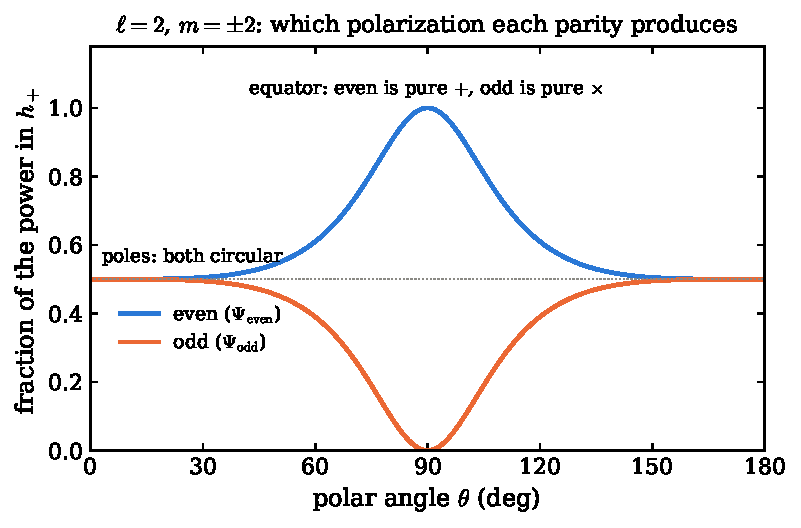
\includegraphics[width=0.62\textwidth]{r4_f01_patterns.pdf}
\caption{Fraction of the radiated power carried by $h_+$ as a function of the polar angle, for an $\ell=2$, $m=\pm2$ wave
of either parity.}\label{fig:patterns}
\end{figure}

\begin{learned}
$h_+$ and $h_\times$ are both built from both parities. The two parities are related by a $45^\circ$ rotation of the
polarization, and they carry energy with equal weight. The natural invariant basis is $(\Psi_{\rm even},\Psi_{\rm odd})$, the
$E/B$ basis, not $(h_+,h_\times)$.
\end{learned}

%==========================================================================================
\section{Can reflection turn $h_\times$ into $h_+$? A selection rule}\label{sec:rule}
\begin{question}
A wave hits the object and comes back. Can a wave that arrives as pure $h_\times$ come back with some $h_+$?
\end{question}

\subsection{Parity is conserved}
\begin{keyidea}
The background (flat interior, shell, Schwarzschild exterior) is spherically symmetric \emph{and} invariant under
parity. The linearized equations therefore commute with rotations and with parity. Modes with different $(\ell,m)$ or
different parity cannot be coupled, to all orders in linear theory and for any spherically symmetric object: black
hole, shell, star.
\end{keyidea}
In the language of the junction conditions, the even and odd systems separate completely: the odd sector involves only
$\Psi_{\rm odd}$, and the even sector only $\Psi_{\rm even}$ and the shell's even degrees of freedom. The response of the
object to each $(\ell,m,{\rm parity})$ channel is a single complex number per frequency, the \emph{reflection amplitude}
\begin{equation}
S_P(\omega)=\frac{B^{P}_{\rm out}}{B^{P}_{\rm in}},\qquad P\in\{{\rm even},{\rm odd}\},
\end{equation}
where $\Psi_P\to B^P_{\rm in}e^{-i\omega r_*}+B^P_{\rm out}e^{+i\omega r_*}$. Both master functions are normalized in the same way
relative to $h$ by Eqs.~\eqref{eq:hplus}--\eqref{eq:hcross}, so the \emph{ratio} $S_{\rm even}/S_{\rm odd}$ is physical.

\subsection{The object as a polarizing mirror}
For one $(\ell,m)$, write the incident wave as a vector in the $E/B$ basis. Reflection acts as a diagonal Jones matrix:
\begin{equation}
\begin{pmatrix}\Psi_{\rm even}\\ \Psi_{\rm odd}\end{pmatrix}_{\rm out}=
\begin{pmatrix}S_{\rm even}&0\\0&S_{\rm odd}\end{pmatrix}\begin{pmatrix}\Psi_{\rm even}\\ \Psi_{\rm odd}\end{pmatrix}_{\rm in}
=S_{\rm odd}\begin{pmatrix}\rho\,e^{i\Phi}&0\\0&1\end{pmatrix}\begin{pmatrix}\Psi_{\rm even}\\ \Psi_{\rm odd}\end{pmatrix}_{\rm in},
\end{equation}
with the \textbf{retardance} $\Phi=\arg(S_{\rm even}/S_{\rm odd})$ and the \textbf{diattenuation} $\rho=|S_{\rm even}/S_{\rm odd}|$.
This is exactly the optics of a birefringent mirror. It gives a precise answer to the question:
\begin{itemize}
\item A wave of \emph{pure parity} keeps its parity. In particular, an axisymmetric ($m=0$) pure-$h_\times$ wave is odd and
\textbf{always comes back as pure $h_\times$}, with a different waveform. No object with spherical symmetry can convert
it into $h_+$.
\item A wave containing \emph{both} parities changes its polarization state, because the two components are reflected
with different phases (and, if the object absorbs, different amplitudes). For a wave incident with equal $E$ and $B$
content ($45^\circ$ linear polarization in the $E/B$ plane, e.g.\ an $m=0$ wave with $h_+=h_\times$), the fraction of the
reflected power found in the orthogonal polarization is, for $\rho=1$,
\begin{equation}
f_{\rm conv}=\sin^2(\Phi/2).
\label{eq:conv}
\end{equation}
The same expression gives the probability that a circularly polarized (helicity) mode comes back with the opposite
helicity, because a helicity state is $\Psi_{\rm even}\pm i\Psi_{\rm odd}$.
\end{itemize}
The rest of the report computes $\Phi(\omega)$ for a black hole and for shells, and shows what it does to waveforms.

%==========================================================================================
\section{Reference case: a black hole is a pure retarder}\label{sec:bh}
\begin{question}
The Regge--Wheeler and Zerilli potentials are different, yet a Schwarzschild black hole has the same QNMs and the same
reflectivity for both parities (isospectrality). Does that mean it treats $h_+$ and $h_\times$ identically?
\end{question}
Isospectrality follows from the Chandrasekhar transformation \cite{Chandrasekhar83}, which maps every solution of the
Regge--Wheeler equation into a solution of the Zerilli equation:
\begin{equation}
\Psi_{\rm even}=\Big[\lambda_\ell+\frac{72M^2f}{r(\mu r+6M)}\Big]\Psi_{\rm odd}+12M\frac{\dd\Psi_{\rm odd}}{\dd r_*},\qquad
\lambda_\ell=\mu(\mu+2)=(\ell-1)\ell(\ell+1)(\ell+2),
\end{equation}
with $\mu=(\ell-1)(\ell+2)$. Take the black-hole scattering solution, which is purely ingoing at the horizon. On the
horizon side $f\to0$, so the map multiplies the ingoing wave by $\lambda_\ell-12iM\omega$ and keeps the boundary condition.
At infinity the extra term vanishes, and the map multiplies $e^{-i\omega r_*}$ by $\lambda_\ell-12iM\omega$ and $e^{+i\omega r_*}$ by
$\lambda_\ell+12iM\omega$. Hence
\begin{equation}
\boxed{\ \frac{S_{\rm even}}{S_{\rm odd}}=\frac{\lambda_\ell+12iM\omega}{\lambda_\ell-12iM\omega}\quad\Longrightarrow\quad
\rho=1,\qquad \Phi_{\rm BH}(\omega)=2\arctan\frac{12M\omega}{(\ell-1)\ell(\ell+1)(\ell+2)}\ }
\label{eq:bhphase}
\end{equation}
The black hole reflects the two parities with the same amplitude (isospectrality) but \emph{not} with the same phase.
It is a pure retarder. We computed $S_{\rm even}$ and $S_{\rm odd}$ independently, by integrating the Zerilli and
Regge--Wheeler equations from the horizon, and recover Eq.~\eqref{eq:bhphase} to better than $5\times10^{-8}$ for
$\ell=2,3,4$ (Fig.~\ref{fig:bhphase}). This also confirms that the numerical normalization of the two parities is
consistent.

For $\ell=2$ ($\lambda_2=24$) the retardance is $21^\circ$ at the fundamental QNM frequency $\omega M=0.374$ and grows to
$90^\circ$ at $\omega M=2$. It is much smaller for higher $\ell$ ($\lambda_3=120$, $\lambda_4=360$). The effect comes entirely
from the exterior Schwarzschild field: it would be the same for \emph{any} compact object at frequencies where the wave does
not reach its surface.

\begin{figure}[h]\centering
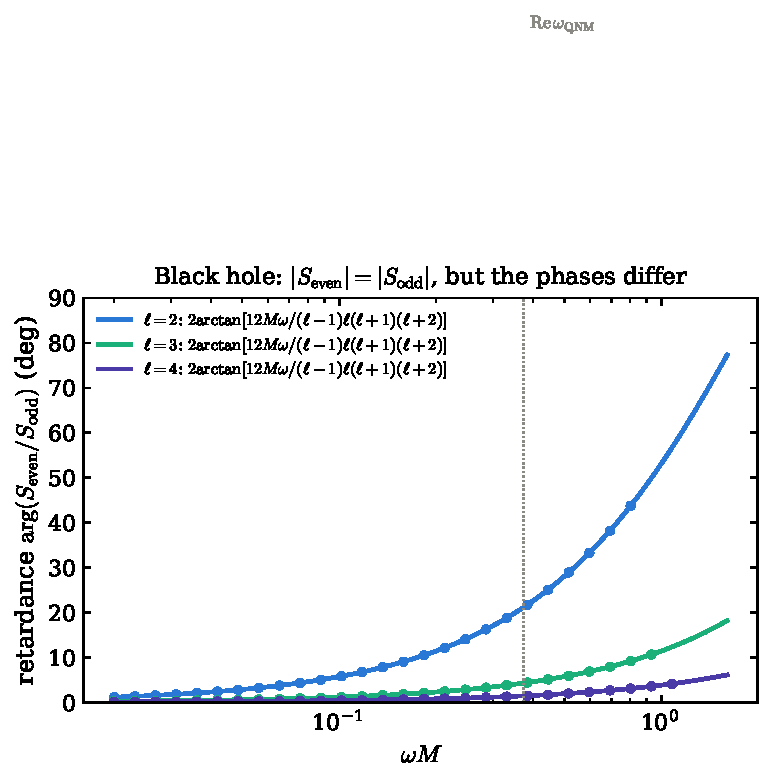
\includegraphics[width=0.62\textwidth]{r4_f02_bh_retardance.pdf}
\caption{Black hole: retardance between the two parities. Lines: Eq.~\eqref{eq:bhphase}. Circles: independent numerical
integration of the two master equations (shown where the reflectivity exceeds $10^{-6}$).}\label{fig:bhphase}
\end{figure}

\begin{learned}
Even a black hole is birefringent. Isospectrality means equal \emph{moduli}, not equal \emph{phases}. A wave that reflects
off the potential barrier comes back with its $E$ and $B$ parts shifted by $\Phi_{\rm BH}$, so its polarization changes.
\end{learned}

%==========================================================================================
\section{The shell as a polarizing mirror}\label{sec:shell}
\begin{question}
The shell has no horizon and absorbs nothing, so $|S_{\rm even}|=|S_{\rm odd}|=1$. How different are the phases, and when
does the polarization change appreciably?
\end{question}
We computed $S_{\rm even}(\omega)$ and $S_{\rm odd}(\omega)$ for $\ell=2$ and $R=6M$, $3M$ and $2.2M$. The physical, regular interior
was carried through the junction conditions and the exterior was integrated to large radius. Near the narrow
resonances the frequency grid was refined adaptively (up to $\sim1400$ frequencies per curve). Numerically
$|S|=1$ holds to $10^{-15}$ in both parities, as it must. Figures~\ref{fig:ret} and \ref{fig:conv} show the retardance
$\Phi=\arg(S_{\rm even}/S_{\rm odd})$ and the converted fraction $\sin^2(\Phi/2)$.

\begin{figure}[t]\centering
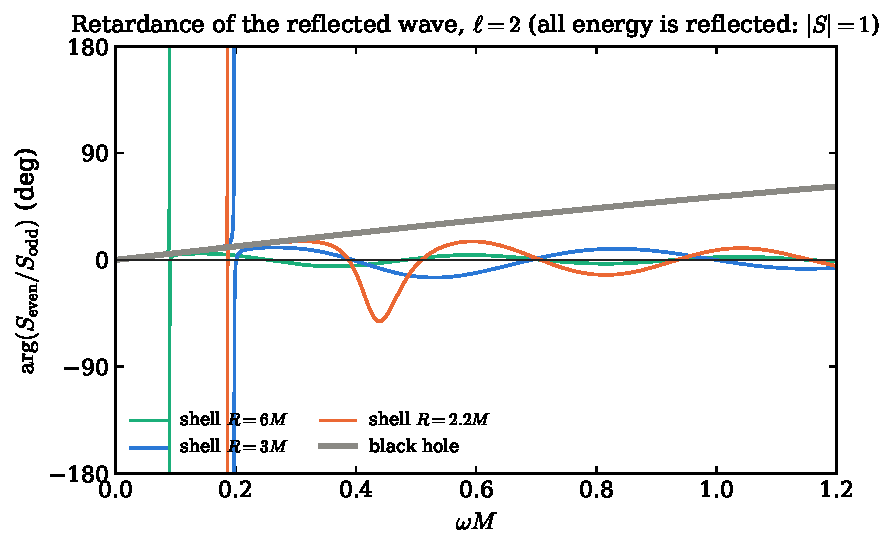
\includegraphics[width=0.49\textwidth]{r4_f03_shell_retardance.pdf}\hfill
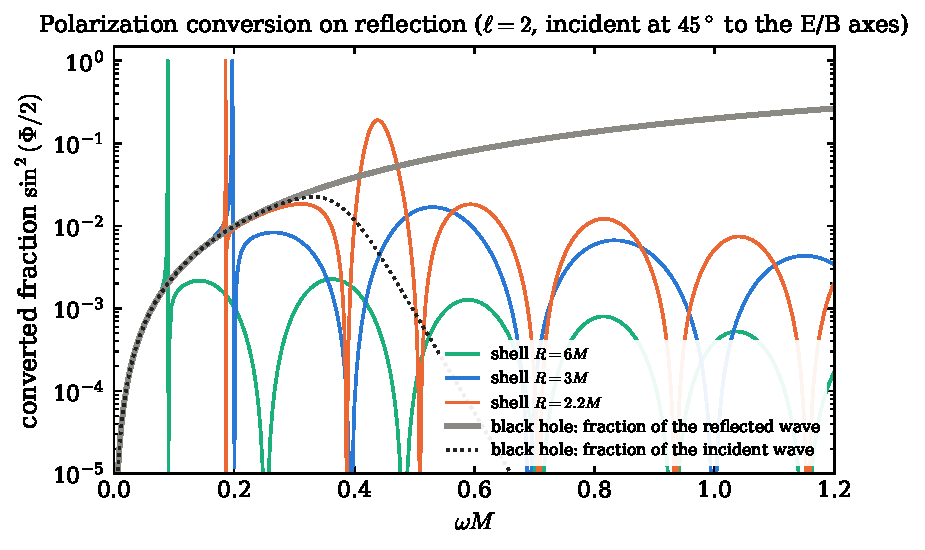
\includegraphics[width=0.49\textwidth]{r4_f04_conversion.pdf}
\caption{Left: retardance between the parities for three shells and the black hole ($\ell=2$). Right: fraction of the
reflected power that comes back in the orthogonal polarization, for a wave with equal $E$ and $B$ content. For the
black hole the dotted line multiplies by the reflectivity, i.e.\ it is the fraction of the \emph{incident} power.}
\label{fig:ret}\label{fig:conv}
\end{figure}

\paragraph{Low frequency: universal.} For $\omega M\lesssim0.1$ all shells follow the black-hole curve
$\Phi=2\arctan(12M\omega/24)$. At $\omega M=0.05$ we find $\Phi=2.86^\circ$ for $R=2.2M$ and $3M$ and $2.84^\circ$ for $6M$, against
$2.86^\circ$ from Eq.~\eqref{eq:bhphase}. Long waves never reach the surface. They are reflected by the exterior
Schwarzschild field, whose even/odd phase difference is fixed by the Chandrasekhar transformation. The structure of the
object enters only at higher order (tidal response).

\paragraph{The matter resonance: complete conversion.} The even sector has a long-lived matter mode, an oscillation of
the shell's fluid, at $\omega M=0.0894-0.00005i$ ($R=6M$), $0.1971-0.0003i$ ($3M$) and $0.1859-0.00003i$ ($2.2M$). The odd sector
has nothing there. Across the resonance the phase of $S_{\rm even}$ winds by $2\pi$ while $S_{\rm odd}$ stays smooth. The
retardance therefore sweeps through $180^\circ$ and the conversion reaches $\sin^2(\Phi/2)=1$: in a narrow band, of width
$\sim|{\rm Im}\,\omega|$, the shell \emph{rotates the polarization of the reflected wave completely}. This is the clearest
answer to ``can $h_\times$ become $h_+$'': an $\ell=2$, $m=\pm2$ wave that arrives as pure $h_\times$ at the equator
(pure odd) comes back as pure $h_\times$. But a wave arriving with equal $E$ and $B$ parts at the matter frequency comes back
with its polarization rotated by $90^\circ$, for instance $h_+=h_\times$ returning as $h_+=-h_\times$.

\paragraph{Intermediate frequencies: small but structured.} Away from the matter resonance the retardance oscillates
around zero. The two parities have cavity and trapped resonances at slightly different frequencies (e.g.\ $0.421-0.035i$
odd and $0.447-0.044i$ even at $R=2.2M$). The frequency-averaged converted fraction on $0.1<\omega M<1$ is $0.08\%$ ($R=6M$),
$0.7\%$ ($3M$) and $1.7\%$ ($2.2M$), with a maximum of $19\%$ between the two trapped resonances of the $R=2.2M$ shell. At high
frequency the wave crosses the transparent shell and bounces off the centre, and both parities acquire the same phase:
$\Phi\to0$.

\paragraph{Contrast with the black hole.} For a black hole the retardance keeps growing with frequency. At high
frequency, however, almost nothing is reflected, so the converted fraction of the \emph{incident} power (dotted curve)
peaks at $\simeq2\%$ near the barrier top and then falls. A shell returns everything, so its polarization
signature can be much stronger (complete, at the matter resonance) but is confined to narrow bands.

\begin{learned}
Parity is conserved, but polarization is not. A compact shell acts as a retarder whose retardance is universal at low
frequency, oscillates at intermediate frequency, and sweeps through $180^\circ$ at the even-only matter resonance, where the
conversion is complete.
\end{learned}

%------------------------------------------------------------------------------------------
\subsection{An absorbing interior: the parities are also reflected with different strength}
If the interior is replaced by a perfect absorber (only an ingoing wave inside, as a horizon would do), the object
also acquires a \emph{diattenuation}: $\RR_{\rm even}\ne\RR_{\rm odd}$ (Fig.~\ref{fig:open}). The two reflectivities coincide at
low and high frequency. Around the barrier top the even parity is reflected more strongly: by a factor of up to $3.4$
($R=2.2M$) and $18$ ($R=6M$), and by a large factor at $R=3M$ near $\omega M\approx0.55$, where the odd reflectivity has an
interference zero. The ratio never drops below $0.98$. The black hole has $\RR_{\rm even}=\RR_{\rm odd}$ exactly. Such a
diattenuating mirror turns an unpolarized wave into a partially polarized one, with an excess of the even ($E$-type)
pattern.

\begin{figure}[h]\centering
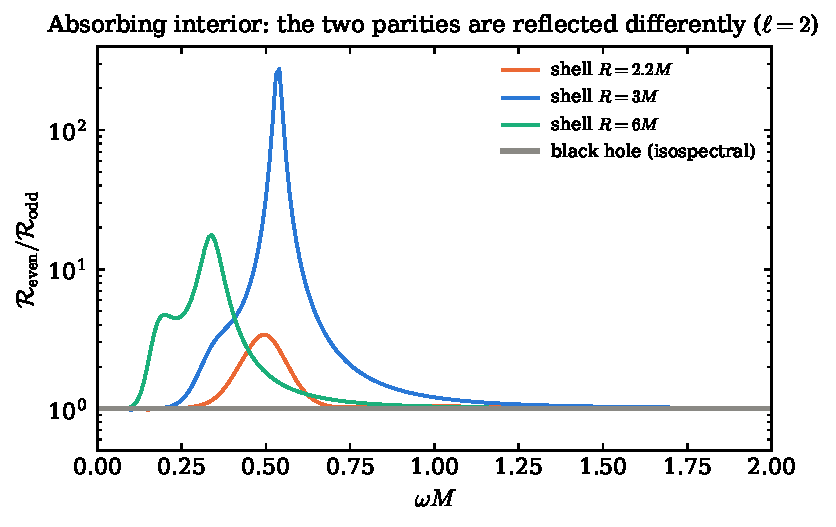
\includegraphics[width=0.6\textwidth]{r4_f12_open_ratio.pdf}
\caption{Ratio of the even to the odd reflectivity when the interior absorbs everything that crosses the shell.}\label{fig:open}
\end{figure}

%==========================================================================================
\section{Plane waves: how much helicity is reversed}\label{sec:plane}
\begin{question}
A distant source sends a circularly polarized plane wave onto the object. What fraction of the scattered radiation has the
opposite helicity?
\end{question}
A plane wave of definite helicity has, for every $\ell\ge2$, equal-magnitude even and odd components combined as
$\Psi_{\rm even}\pm i\Psi_{\rm odd}$. After scattering, the helicity-preserving amplitude of partial wave $\ell$ is
$(S_{\rm even}+S_{\rm odd})/2-1$ and the helicity-reversing amplitude is $(S_{\rm even}-S_{\rm odd})/2$. By orthogonality of the
spin-weighted harmonics the helicity-reversing cross section is
\begin{equation}
\sigma_{\rm flip}(\omega)=\frac{\pi}{\omega^2}\sum_{\ell\ge2}(2\ell+1)\,\frac{|S^\ell_{\rm even}-S^\ell_{\rm odd}|^2}{4}.
\label{eq:sflip}
\end{equation}
Unlike the total cross section, which diverges because of the long-range Newtonian potential, $\sigma_{\rm flip}$ is
\emph{finite}. The Newtonian phase is common to both parities and cancels in the difference.

\paragraph{Black hole, exactly.} With Eq.~\eqref{eq:bhphase}, $|S_{\rm even}-S_{\rm odd}|^2/4=\RR_\ell\sin^2\arctan(12M\omega/\lambda_\ell)$,
where $\RR_\ell$ is the reflectivity of partial wave $\ell$. As $\omega\to0$, $\RR_\ell\to1$ and
\begin{equation}
\sigma_{\rm flip}\to144\pi M^2\sum_{\ell\ge2}\frac{2\ell+1}{[(\ell-1)\ell(\ell+1)(\ell+2)]^2}=144\pi M^2\cdot\frac1{108}=\frac{4\pi}{3}M^2 .
\label{eq:4pi3}
\end{equation}
The sum can be done in closed form (symbolic summation gives exactly $1/108$). The result coincides with the angular integral of the
helicity-reversing part, $M^2\sin^4(\theta/2)$, of the classic long-wavelength cross section
$\dd\sigma/\dd\Omega=M^2[\cos^8(\theta/2)+\sin^8(\theta/2)]/\sin^4(\theta/2)$ \cite{Peters76,DeLogi77,FHM88,Dolan08}:
$\int M^2\sin^4(\theta/2)\,\dd\Omega=4\pi M^2/3$. The partial-wave formalism, the relative normalization of the two parities
and the Chandrasekhar phase are therefore all consistent with the known result.

\paragraph{Shells.} Evaluating Eq.~\eqref{eq:sflip} numerically ($\ell$ up to $\sim2.2\,\omega R+7$, last term below
$5\times10^{-4}$ of the sum) gives Fig.~\ref{fig:sflip}. At $\omega M=0.02$ all objects give $\sigma_{\rm flip}=4.188M^2$, the
universal value~\eqref{eq:4pi3}. The helicity flip at long wavelengths depends only on the mass. At higher frequency the
curves separate. The dilute shell ($R=6M$) flips less than a black hole around $\omega M\sim0.1$--$0.5$, because its partial
waves pass through the shell and the centre almost symmetrically. The compact shells flip more than the black hole for $\omega M\gtrsim0.4$, where the black hole absorbs almost everything, and
the $R=2.2M$ shell shows sharp peaks (up to $\sim24M^2$ on our grid) at the trapped resonances of the higher multipoles.
These peaks are only partly resolved by the frequency grid.

\begin{figure}[h]\centering
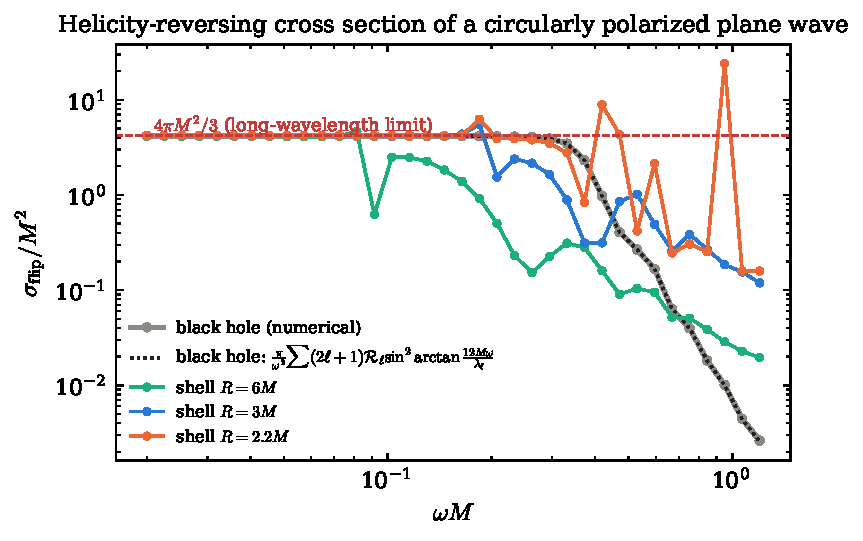
\includegraphics[width=0.66\textwidth]{r4_f05_sigma_flip.pdf}
\caption{Helicity-reversing cross section, Eq.~\eqref{eq:sflip}, for the black hole (numerical, and the closed form with
numerical reflectivities) and three shells. Dashed: the universal long-wavelength value $4\pi M^2/3$.}\label{fig:sflip}
\end{figure}

\begin{learned}
Any spherical compact object reverses the helicity of long gravitational waves with cross section $4\pi M^2/3$,
independent of its structure. Structure-dependent polarization signatures appear at $\omega\sim1/R$ and are strongest near
resonances.
\end{learned}

%==========================================================================================
\section{Waveforms: the same incident $h_+$ pulse in the two parities}\label{sec:time}
\begin{question}
What does a detector see if the same pulse arrives once carried by the even master function and once by the odd one?
\end{question}
\paragraph{Set-up.} For a single $(\ell,m)$ the angular factor in Eq.~\eqref{eq:spin} is the same for the incident and the
reflected wave. So $h_+$ and $h_\times$ at any fixed direction are that angular factor times $\Psi_{\rm in}(v)$ before the
reflection and $\Psi_{\rm out}(u)$ after it. For instance, for $m=0$ the even channel is literally ``incident $h_+$, reflected
$h_+$'', and the odd channel is the same with $h_\times$. We therefore compare the reflected $\Psi_{\rm out}(u)$ of the two
parities for the same incident pulse,
\begin{equation}
\Psi_{\rm in}(v)=e^{-v^2/2\sigma^2}\cos(\omega_0v),\qquad \sigma=8M,\quad \omega_0=0.5/M,\qquad v=t+r_* ,
\end{equation}
by Fourier synthesis, $\Psi_{\rm out}(u)=\frac1{2\pi}\int S(\omega)\tilde\Psi_{\rm in}(\omega)e^{-i\omega u}\dd\omega$, with $u=t-r_*$. The
integral is done with a Filon-type quadrature on the adaptive frequency grid, so the narrow resonances are resolved.

\paragraph{Causality and the instability.} The fluid shell has an unstable even-parity matter mode at $\omega=i\gamma$.
There, $S_{\rm even}$ has a pole in the upper half plane, and the real-axis integral is then \emph{not} the causal response.
The causal (retarded) response is obtained by moving the contour above the pole:
\begin{equation}
\Psi^{\rm causal}_{\rm out}(u)=\Psi^{\rm real\ axis}_{\rm out}(u)-i\,{\rm Res}_{\omega=i\gamma}\big[S_{\rm even}\tilde\Psi_{\rm in}\big]\,e^{\gamma u}.
\end{equation}
The residue must be computed directly. For ${\rm Im}\,\omega>0$ the outgoing solution decays with $r$, so we project the
exterior solution onto the in/out asymptotic solutions at a moderate radius. This reproduces the real-axis $S$ to
$10^{-8}$, and Newton iteration on $B_{\rm in}=0$ returns the pole exactly at the known unstable frequency:
$0.1332058i$ ($R=3M$), $0.2442921i$ ($2.2M$), $0.0401379i$ ($6M$). The residues, stable to three digits against the
projection radius, are tiny: $7.5\times10^{-5}i$, $8.2\times10^{-6}i$ and $1.1\times10^{-5}i$. The unstable mode lives in the
shell's matter and is only weakly coupled to waves coming from infinity. For this pulse its amplitude at $u=0$ is
$3.9\times10^{-7}$ ($R=3M$), $1.4\times10^{-8}$ ($2.2M$) and $2.3\times10^{-8}$ ($6M$). It reaches the amplitude of the incident
pulse at $u\approx111M$, $74M$ and $438M$ respectively.

\paragraph{Check.} For the odd channel the result was compared with a direct time-domain (leapfrog) evolution of
$\partial_t^2\Psi=\partial_x^2\Psi-V\Psi-\Delta\,\delta(x-x_R)\Psi$ that shares no code with the frequency-domain calculation. With
source and detector far from the object ($x=450M$ and $350M$), and the $O(1/\omega r)$ near-zone factors of the in/out
solutions included, the two agree to $0.4\%$ ($R=3M$) and $0.9\%$ ($2.2M$) of the peak (Fig.~\ref{fig:lf}).

\begin{figure}[p]\centering
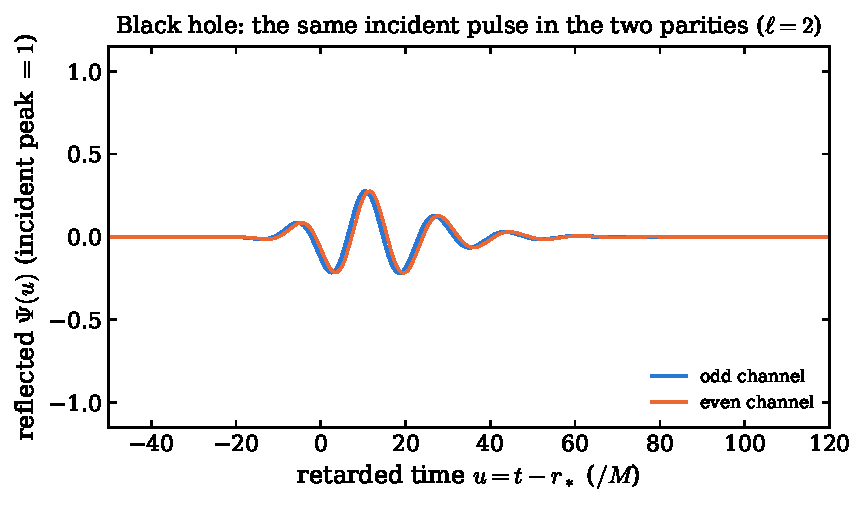
\includegraphics[width=0.49\textwidth]{r4_f06_time_bh.pdf}\hfill
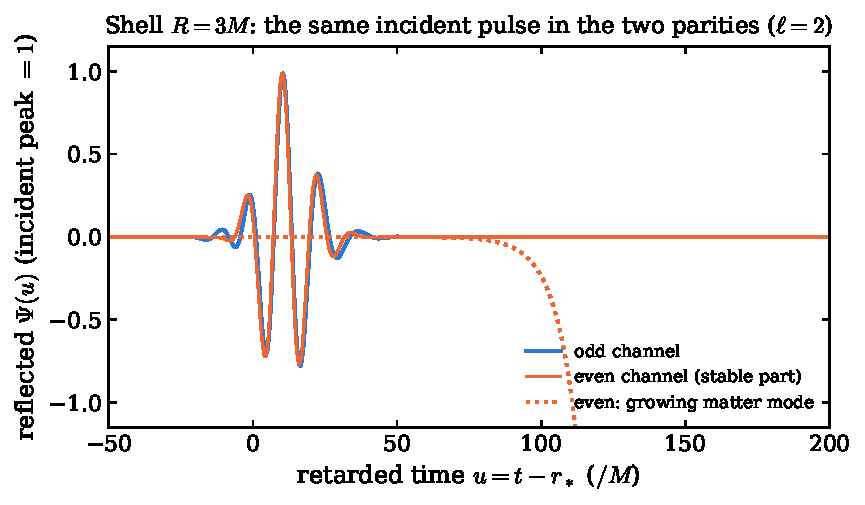
\includegraphics[width=0.49\textwidth]{r4_f07_time_R3.pdf}\\[2mm]
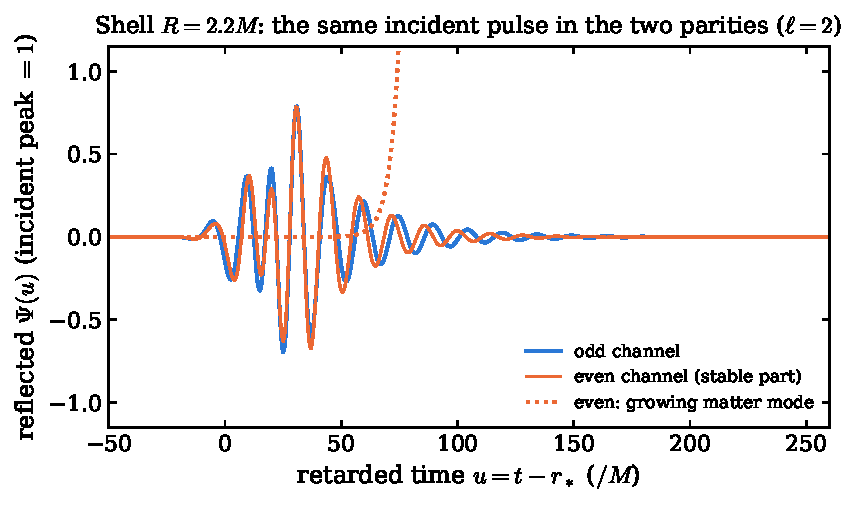
\includegraphics[width=0.49\textwidth]{r4_f08_time_R22.pdf}\hfill
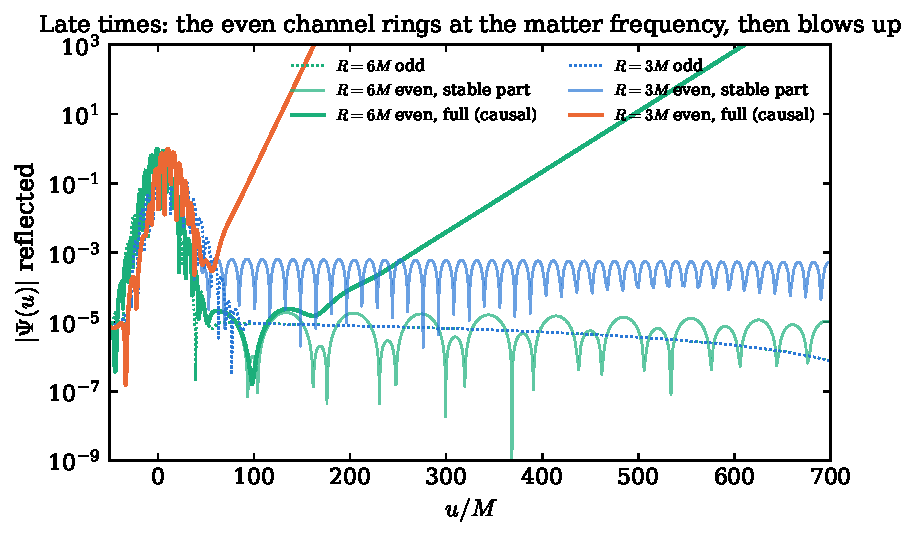
\includegraphics[width=0.49\textwidth]{r4_f09_time_log.pdf}
\caption{Reflected waveforms of the same incident pulse, carried by the odd (blue) or even (orange) master function. Top
left: black hole. Top right: shell at $3M$. Bottom left: shell at $2.2M$. Dotted: the growing matter mode of the even
channel, added causally. Bottom right: long-time view (log scale) for $R=6M$ and $3M$. The even channel keeps ringing at
the matter frequency and is eventually overtaken by the unstable mode; the odd channel just decays. The floor at
$\sim10^{-5}$ is numerical.}\label{fig:time}
\end{figure}

\paragraph{What the waveforms show (Fig.~\ref{fig:time}).}
\begin{itemize}
\item \textbf{Black hole.} The two waveforms are almost identical. The even one is the odd one passed through the
all-pass filter $(\lambda_\ell-12M\partial_u)/(\lambda_\ell+12M\partial_u)$, the time-domain form of Eq.~\eqref{eq:bhphase}. This
gives a delay of $\simeq24M/\lambda_\ell=1M$ for $\ell=2$ at low frequency. Both ring down at the same QNM.
\item \textbf{Shell at $3M$.} The prompt reflection is again nearly the same in both parities (the retardance is only
$\sim10^\circ$ in this band). The difference is at late times: the even channel keeps a weak ringing at the matter frequency
$\omega M=0.197$, with a decay time $\sim3000M$. On top of it the unstable mode grows as $e^{0.133u/M}$ and dominates after
$\sim110M$. The odd channel has neither.
\item \textbf{Shell at $2.2M$.} Both parities ring in their trapped modes, at slightly different frequencies ($0.421$ odd,
$0.447$ even) and dampings ($0.035$ vs $0.044$). The two waveforms dephase visibly after a few cycles, and the unstable
mode takes over the even channel after $\sim74M$.
\item \textbf{Shell at $6M$.} The prompt reflections are indistinguishable. The even channel carries a long matter
ringing at $\omega M=0.089$ at the $10^{-5}$ level and blows up after $\sim440M$.
\end{itemize}

\paragraph{Polarization in the time domain.} For a pulse with equal $E$ and $B$ content, the part that comes back with the
orthogonal polarization is $(\Psi^{\rm even}_{\rm out}-\Psi^{\rm odd}_{\rm out})/2$ (Fig.~\ref{fig:rot}). It carries $3.7\%$ of the
reflected energy for the black hole and $1.0\%$ for the $R=3M$ shell (stable part), concentrated at the edges of the pulse,
where the phase difference acts. In the shell case the rotated component then persists at late times, carried by the
even-only matter ringing.

\begin{figure}[h]\centering
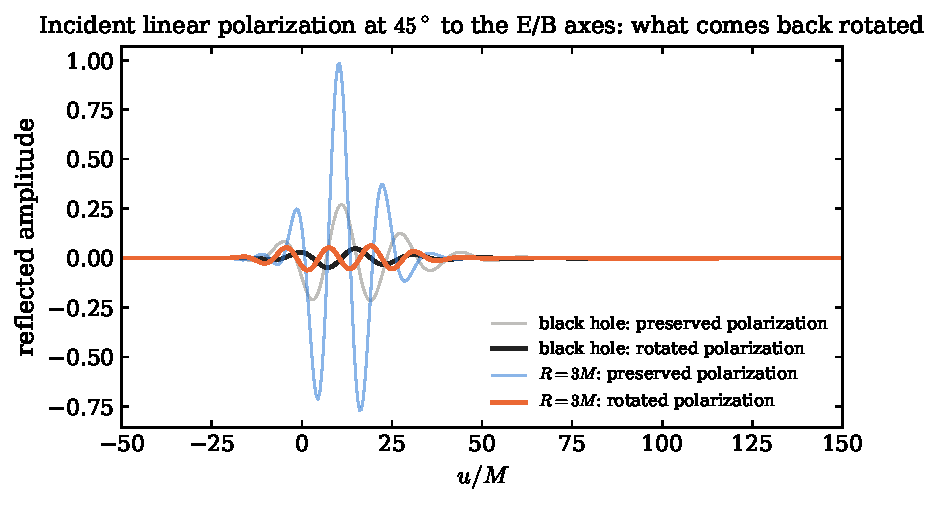
\includegraphics[width=0.49\textwidth]{r4_f10_converted_time.pdf}\hfill
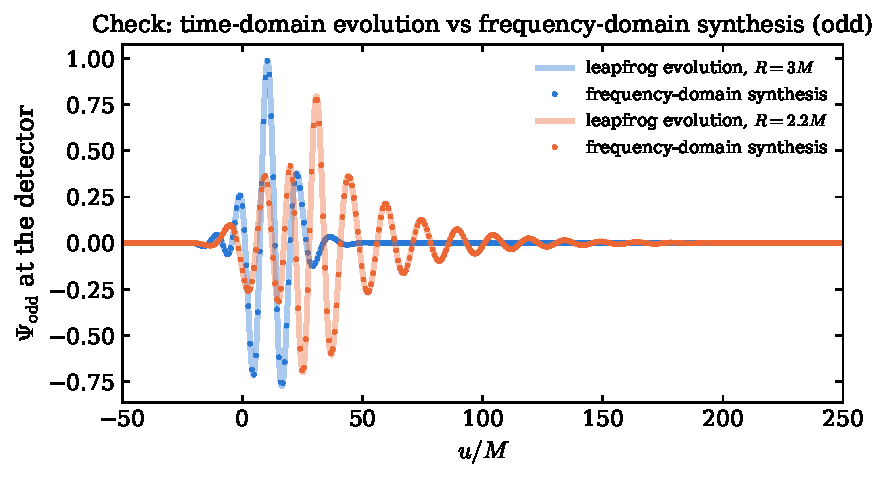
\includegraphics[width=0.49\textwidth]{r4_f11_leapfrog_check.pdf}
\caption{Left: preserved and rotated parts of a reflected pulse with equal $E$ and $B$ content. Right: check of the
frequency-domain synthesis against an independent time-domain evolution (odd channel).}\label{fig:rot}\label{fig:lf}
\end{figure}

\begin{learned}
Plotted as $h_+(t)$, the even and odd reflections of the same pulse look alike during the prompt response. Their
difference grows with time: in the dephasing of the trapped modes, in the even-only matter ringing, and above all in the
even-only instability of the static shell.
\end{learned}

%==========================================================================================
\section{So, is one parity more important?}\label{sec:which}
\begin{question}
For a harder problem one would like to know whether one parity can be neglected. What do the results say?
\end{question}
The answer depends on which of three questions is being asked.

\paragraph{1. Kinematics: no.} The two parities carry energy with identical weights, Eq.~\eqref{eq:flux}, and they are
exchanged by a $45^\circ$ rotation of the polarization. A plane gravitational wave contains equal amounts of both: its
partial-wave expansion has $\Psi^{\ell,\pm2}_{\rm odd}=\pm i\,\Psi^{\ell,\pm2}_{\rm even}$ for every $\ell$. For \emph{scattering of an
external wave} both parities are equally excited, and dropping one loses half of the signal and all of the
polarization physics of Secs.~\ref{sec:shell}--\ref{sec:time}.

\paragraph{2. Response of the object: comparable in energy, different in phase and in physics.}
\begin{itemize}
\item For a non-absorbing object (the shell) $|S_{\rm even}|=|S_{\rm odd}|=1$. Both parities return exactly the energy they
bring. For a black hole the moduli are equal by isospectrality. With an absorbing (``open'') interior the two
reflectivities differ only at intermediate frequencies, near the barrier top, and coincide at low and high frequency.
\item What differs is the \emph{phase} and therefore the \emph{time structure}: the retardance, the ringing frequencies and
their damping (Secs.~\ref{sec:shell}, \ref{sec:time}).
\item Qualitatively, only the even sector \emph{moves the shell and couples to its matter}: radial displacement,
compression and the equation of state all enter through $\Psi_{\rm even}$. The odd sector sees a universal $\delta$-barrier,
$[\partial_x\Psi]=\Delta\Psi$ with $\Delta=\sqrt{f_R}(1-\sqrt{f_R})/R$, which does not depend on the frequency or on the
equation of state. The matter resonances, their long ringing, and the instability of the static shell exist
\emph{only} in the even sector.
\end{itemize}

\paragraph{3. Sources: even dominates for slow sources.} For a source with internal velocities $v\ll1$, the even
$\ell=2$ mode is the mass quadrupole and the odd $\ell=2$ mode is the current quadrupole \cite{Thorne80}. The latter is
suppressed by one power of $v$ in amplitude. For a circular binary of masses $m_1,m_2$ and total mass $m$, the post-Newtonian
flux gives \cite{Blanchet14}
\begin{equation}
\frac{\dot E_{\rm odd,\ \ell=2}}{\dot E_{\rm even,\ \ell=2}}\simeq\frac{1}{36}\Big(\frac{m_1-m_2}{m}\Big)^2v^2 ,
\end{equation}
of the same order as the even $\ell=3$ (mass-octupole) contribution. A radially infalling or head-on source is
axisymmetric and polar and excites \emph{only} the even sector. Odd parity is dominant only for sources driven by
currents: rotation, toroidal flows, or axial (``$w$-mode'' or $r$-mode-like) oscillations.

\begin{keyidea}
Advice for a harder problem. (i) If the problem is the scattering of an external wave, keep both parities. They carry equal
energy, and the polarization of the outgoing wave is set by their relative phase. (ii) If the waves are generated by slow
matter motion, the even sector dominates and the odd sector is an $O(v^2)$ correction in power. (iii) In either case the
odd sector is the \emph{simpler} and more universal one: for a thin shell it reduces to a $\delta$-barrier. It is a
good first test of the code, while the even sector contains the matter physics and the possible instabilities.
\end{keyidea}

%==========================================================================================
\section{Conclusions}\label{sec:concl}
\begin{enumerate}
\item \textbf{Polarizations vs parities.} $h_+-ih_\times=\frac1{2r}\sum\sqrt{(\ell+2)!/(\ell-2)!}\,(\Psi_{\rm even}-i\Psi_{\rm odd})\,{}_{-2}Y^{\ell m}$. The even
and odd master functions are $E$- and $B$-type patterns related by a $45^\circ$ rotation of the polarization. Each
contributes to both $h_+$ and $h_\times$; only for $m=0$ is even $=+$ and odd $=\times$.
\item \textbf{Selection rule.} Spherical symmetry and parity forbid even--odd mixing for any spherical object. A wave of
pure parity keeps its parity: an axisymmetric $h_\times$ wave cannot come back as $h_+$.
\item \textbf{Birefringent mirror.} A wave containing both parities does change polarization, because
$S_{\rm even}\ne S_{\rm odd}$. A black hole is a pure retarder with $\Phi=2\arctan[12M\omega/(\ell-1)\ell(\ell+1)(\ell+2)]$, exactly,
from the Chandrasekhar transformation (verified numerically to $5\times10^{-8}$).
\item \textbf{Universal long-wavelength helicity flip.} $\sigma_{\rm flip}\to4\pi M^2/3$ for any spherical compact object. We
derived this from a partial-wave sum that equals $1/108$ exactly, and it agrees with the classic Schwarzschild cross
section.
\item \textbf{Shell-specific polarization effects.} Complete polarization conversion occurs in narrow bands at the even-only
matter resonance. Conversions of a few per cent (up to $19\%$ for $R=2.2M$) occur between the even and odd trapped
resonances. With an absorbing interior, the even parity is reflected up to an order of magnitude more strongly near the
barrier top.
\item \textbf{Waveforms.} The same incident pulse gives nearly identical prompt reflections in the two parities. The even
channel differs at late times: dephased trapped ringing, a long ringing at the matter frequency, and the growing unstable
mode. The latter is weakly excited (residue $\sim10^{-5}$) but dominates after $\sim74$--$440M$, depending on $R$.
\item \textbf{Which parity matters.} In energy neither: the weights are equal, a plane wave contains both equally, and the
reflected energies are equal for a non-absorbing object. In physics, the even parity carries all the coupling to the
matter and is the dominant emission channel of slow sources. The odd parity is simpler and universal, a $\delta$-barrier.
\end{enumerate}

\paragraph{Methods and checks.} Reflection amplitudes come from the exact junction conditions of the shell (odd: analytic;
even: $2\times2$ matrix from the linearized Israel equations), a regular flat interior, and high-accuracy integration of the
Regge--Wheeler and Zerilli equations. The checks are:
\begin{itemize}
\item the black-hole phase ratio against the Chandrasekhar formula ($5\times10^{-8}$);
\item $|S|=1$ for the shells ($10^{-15}$);
\item the universal low-frequency retardance and helicity-flip cross section;
\item the unstable-pole position against the known matter mode (seven digits);
\item the odd-channel waveforms against an independent time-domain evolution ($<1\%$).
\end{itemize}

\paragraph{Code.} \texttt{code/parity\_study.py}: all computations, cached in \texttt{data/}. \texttt{code/residue.py}:
residue of $S_{\rm even}$ at the unstable pole. \texttt{code/make\_figures\_r4.py}: figures; numbers quoted in the text are in
\texttt{code/numbers\_r4.json}.


%==========================================================================================
\begin{thebibliography}{99}\small
\bibitem{RW57} T.~Regge and J.~A.~Wheeler, Stability of a Schwarzschild singularity, Phys.\ Rev.\ \textbf{108}, 1063 (1957).
\bibitem{Zerilli70} F.~J.~Zerilli, Effective potential for even-parity Regge--Wheeler gravitational perturbation equations, Phys.\ Rev.\ Lett.\ \textbf{24}, 737 (1970).
\bibitem{Vishveshwara70} C.~V.~Vishveshwara, Scattering of gravitational radiation by a Schwarzschild black-hole, Nature \textbf{227}, 936 (1970).
\bibitem{MP05} K.~Martel and E.~Poisson, Gravitational perturbations of the Schwarzschild spacetime: a practical covariant and gauge-invariant formalism, Phys.\ Rev.\ D \textbf{71}, 104003 (2005); K.~Martel, PhD thesis, University of Guelph (2004).
\bibitem{IS84} J.~Ipser and P.~Sikivie, Gravitationally repulsive domain wall, Phys.\ Rev.\ D \textbf{30}, 712 (1984).
\bibitem{Poisson04} E.~Poisson, \emph{A Relativist's Toolkit} (Cambridge University Press, 2004).
\bibitem{Israel66} W.~Israel, Singular hypersurfaces and thin shells in general relativity, Nuovo Cimento B \textbf{44}, 1 (1966).
\bibitem{PSP26} T.~Pitre, B.~Schneider and E.~Poisson, Self-gravitating thin shells are dynamically unstable on all angular scales, Phys.\ Rev.\ D \textbf{113}, 124055 (2026).
\bibitem{Pani09} P.~Pani, E.~Berti, V.~Cardoso, Y.~Chen and R.~Norte, Gravitational wave signatures of the absence of an event horizon. I. Nonradial oscillations of a thin-shell gravastar, Phys.\ Rev.\ D \textbf{80}, 124047 (2009).
\bibitem{Boyanov25} V.~Boyanov, V.~Cardoso, K.~D.~Kokkotas and J.~Redondo-Yuste, Dynamical response of viscous objects to gravitational waves, Phys.\ Rev.\ Lett.\ \textbf{135}, 151402 (2025).
\bibitem{Chandrasekhar83} S.~Chandrasekhar, \emph{The Mathematical Theory of Black Holes} (Oxford University Press, 1983), Ch.~4.
\bibitem{Goldberg67} J.~N.~Goldberg, A.~J.~MacFarlane, E.~T.~Newman, F.~Rohrlich and E.~C.~G.~Sudarshan, Spin-$s$ spherical harmonics and $\eth$, J.\ Math.\ Phys.\ \textbf{8}, 2155 (1967).
\bibitem{Thorne80} K.~S.~Thorne, Multipole expansions of gravitational radiation, Rev.\ Mod.\ Phys.\ \textbf{52}, 299 (1980).
\bibitem{Blanchet14} L.~Blanchet, Gravitational radiation from post-Newtonian sources and inspiralling compact binaries, Living Rev.\ Relativ.\ \textbf{17}, 2 (2014).
\bibitem{FHM88} J.~A.~H.~Futterman, F.~A.~Handler and R.~A.~Matzner, \emph{Scattering from Black Holes} (Cambridge University Press, 1988).
\bibitem{Peters76} P.~C.~Peters, Differential gravitational scattering cross section, Phys.\ Rev.\ D \textbf{13}, 775 (1976).
\bibitem{DeLogi77} W.~K.~De~Logi and S.~J.~Kov\'acs, Gravitational scattering of zero-rest-mass plane waves, Phys.\ Rev.\ D \textbf{16}, 237 (1977).
\bibitem{Dolan08} S.~R.~Dolan, Scattering and absorption of gravitational plane waves by rotating black holes, Class.\ Quantum Grav.\ \textbf{25}, 235002 (2008).
\bibitem{Leaver85} E.~W.~Leaver, An analytic representation for the quasi-normal modes of Kerr black holes, Proc.\ R.\ Soc.\ Lond.\ A \textbf{402}, 285 (1985).
\bibitem{Cardoso2016PRL} V.~Cardoso, E.~Franzin and P.~Pani, Is the gravitational-wave ringdown a probe of the event horizon?, Phys.\ Rev.\ Lett.\ \textbf{116}, 171101 (2016).
\bibitem{CardosoPani2019} V.~Cardoso and P.~Pani, Testing the nature of dark compact objects: a status report, Living Rev.\ Relativ.\ \textbf{22}, 4 (2019).
\bibitem{Kamionkowski97} M.~Kamionkowski, A.~Kosowsky and A.~Stebbins, Statistics of cosmic microwave background polarization, Phys.\ Rev.\ D \textbf{55}, 7368 (1997).
\end{thebibliography}
\end{document}
